\documentclass[12pt,a4paper,landscape]{article}

% -- Package Imports --
\usepackage[utf8]{inputenc}
\usepackage[T1]{fontenc}
\usepackage{booktabs}
\usepackage{graphicx}
\graphicspath{{./}{./images/}{../sections/images/}}
\usepackage{longtable}
\usepackage{newtxtext} % Times-like text font
\usepackage{newtxmath} % Times-like math
\usepackage{setspace}
\usepackage{array}
\usepackage{multirow}
\usepackage{tabularx}
\usepackage{xcolor}
\usepackage{colortbl}
\usepackage{geometry}
\usepackage[colorlinks=true,linkcolor=blue,citecolor=blue,urlcolor=blue]{hyperref}
\usepackage{float}
\usepackage{enumitem}
\usepackage{fancyhdr}
\usepackage{pdflscape}
\usepackage{makecell}
\usepackage{caption}

% -- Document Setup --
\geometry{a4paper, margin=2.5cm, landscape}
\setstretch{1.5}
\setlength{\parindent}{0pt}
\setlength{\parskip}{6pt}
\setlength{\headheight}{15pt} % Fix for fancyhdr warning

% -- Table Column Types --
\newcolumntype{L}[1]{>{\raggedright\arraybackslash}p{#1}}
\newcolumntype{C}[1]{>{\centering\arraybackslash}p{#1}}
\newcolumntype{R}[1]{>{\raggedleft\arraybackslash}p{#1}}

% -- Header and Footer --
\pagestyle{fancy}
\fancyhf{}
\fancyhead[L]{PhD Protocol Appendices}
\fancyhead[R]{Craig Parker}
\fancyfoot[C]{Page \thepage}
\renewcommand{\headrulewidth}{0.4pt}
\renewcommand{\footrulewidth}{0.4pt}

\begin{document}

\begin{center}
    \Large\textbf{APPENDICES}\\[0.5em]
    \large\textbf{Urban Heat, Health, and Vulnerability in South African Cities:}\\
    \large\textbf{A Mixed-Methods Approach to Predictive Modeling}\\[0.5em]
    \normalsize Craig Parker\\
    \normalsize University of Cape Town\\
    \normalsize April 2025
\end{center}

\section*{Appendix A: Supplementary Figures}

\subsection*{A.1 Temperature Trends in Johannesburg}
\begin{figure}[H]
    \centering
    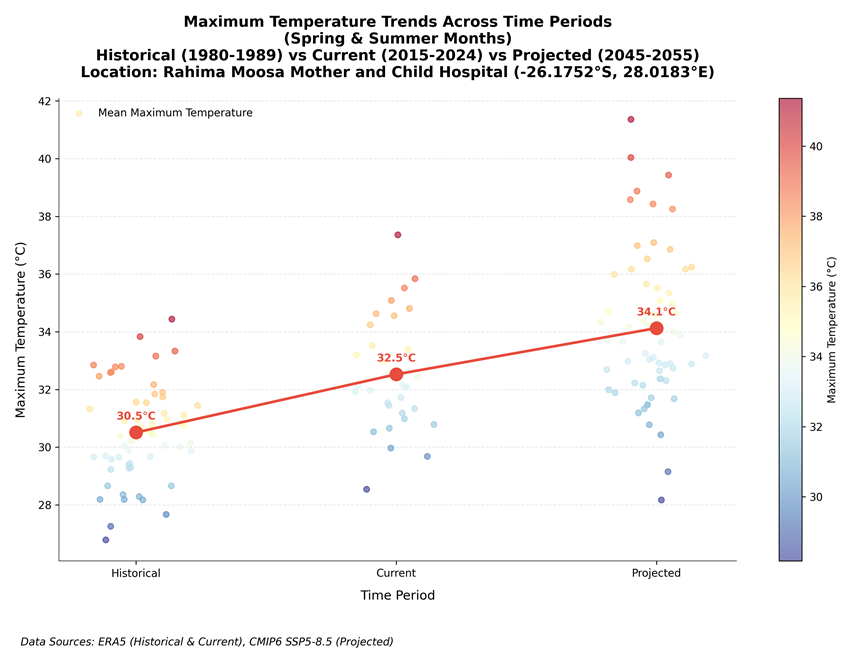
\includegraphics[width=0.8\textwidth]{images/Max_temp_trends_across_time_periods.png}
    \caption{Maximum temperature trends across different time periods in Johannesburg, showing increasing frequency and intensity of extreme heat events.}
    \label{fig:temp_trends}
\end{figure}

\subsection*{A.2 Seasonal Heat Patterns}
\begin{figure}[H]
    \centering
    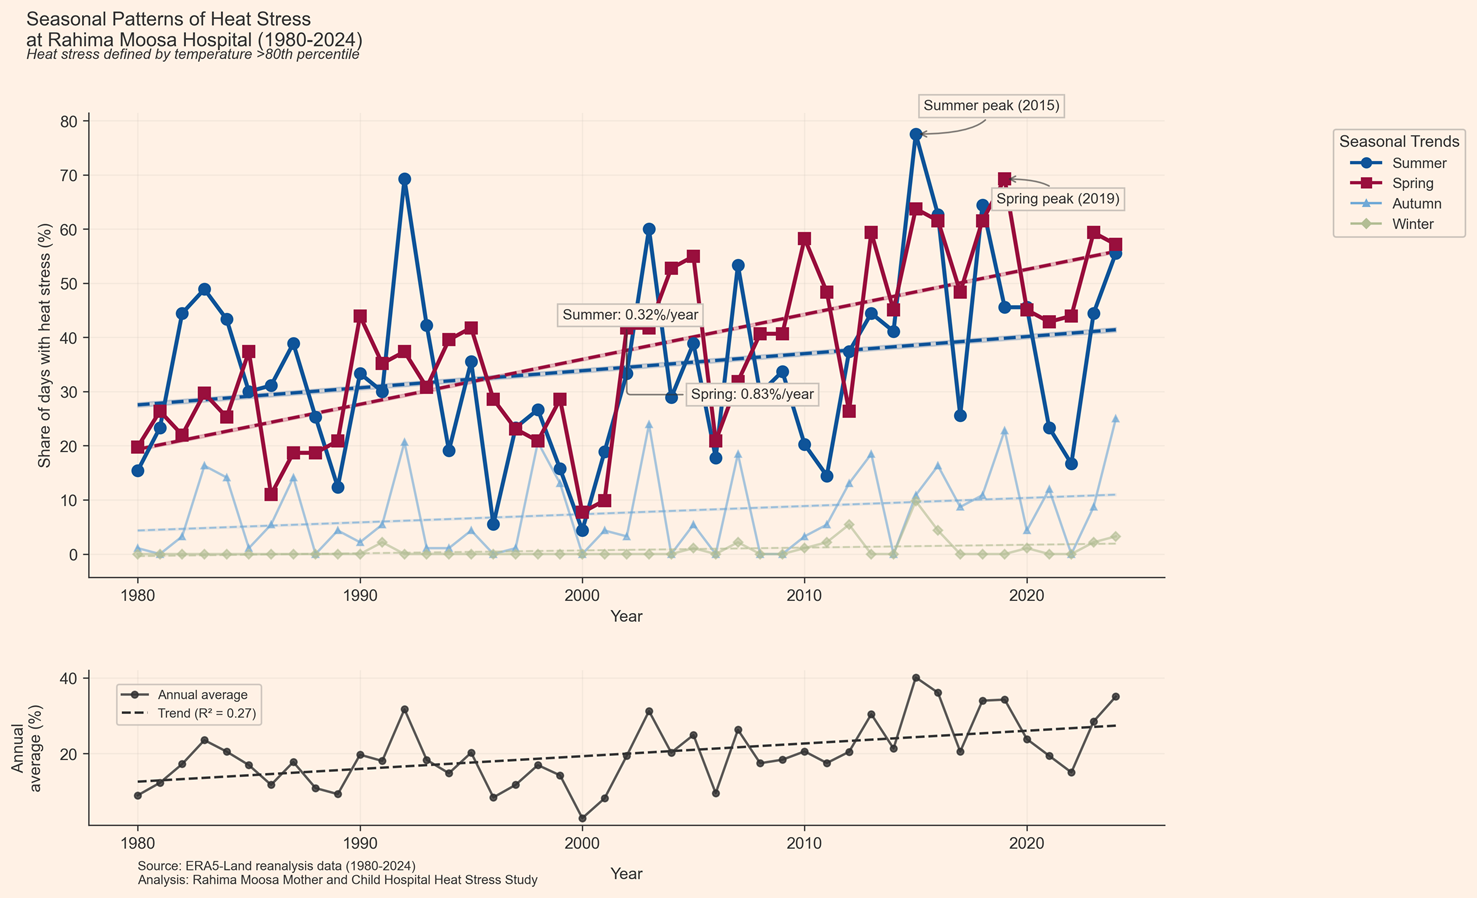
\includegraphics[width=0.8\textwidth]{images/seasonal_heat_Rahima_1980_2024.png}
    \caption{Seasonal heat patterns in the Johannesburg region from 1980-2024, highlighting increasing summer temperature extremes.}
    \label{fig:seasonal}
\end{figure}

\subsection*{A.3 Global Temperature Comparison}
\begin{figure}[H]
    \centering
    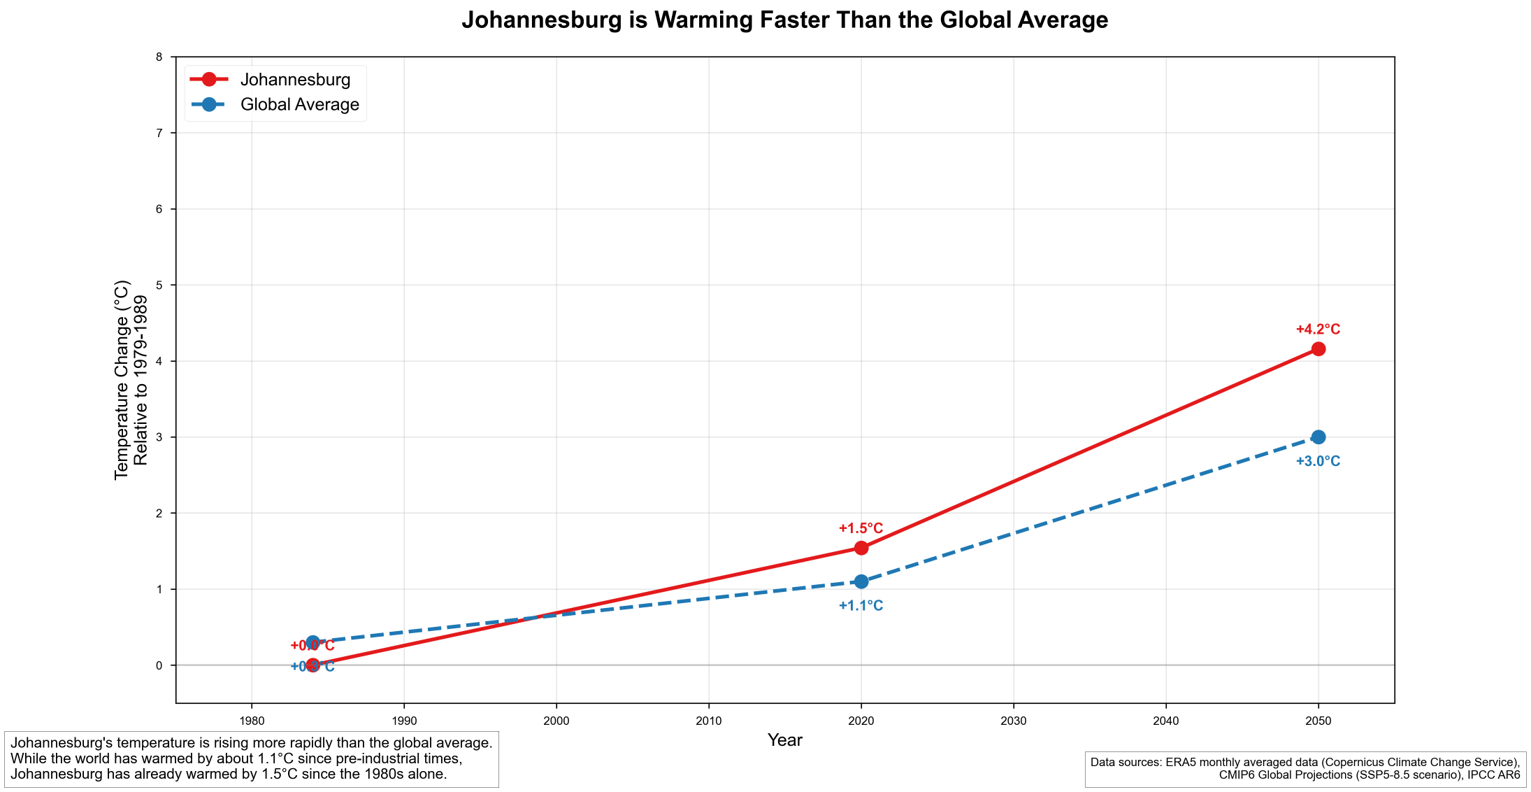
\includegraphics[width=0.8\textwidth]{images/global_temp_versus_Johannesburg.png}
    \caption{Comparison of global temperature anomalies versus Johannesburg-specific trends, showing amplified urban warming.}
    \label{fig:global_comparison}
\end{figure}

\subsection*{A.4 Urban Heat Island Analysis}
\begin{figure}[H]
    \centering
    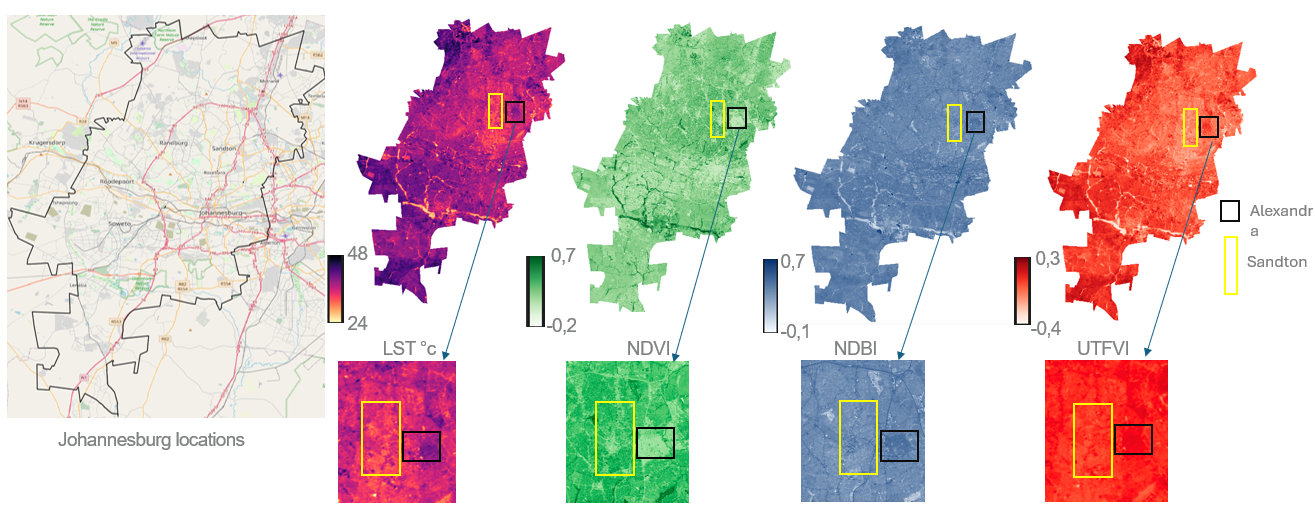
\includegraphics[width=0.8\textwidth]{images/heat_stress_LST_NDVI_NDBI_UTFVI_Johannesburg.png}
    \caption{Urban heat island analysis using land surface temperature (LST), vegetation index (NDVI), built-up index (NDBI), and urban thermal field variance index (UTFVI) for Johannesburg.}
    \label{fig:uhi}
\end{figure}

\subsection*{A.5 Preliminary Heat Vulnerability Index}
\begin{figure}[H]
    \centering
    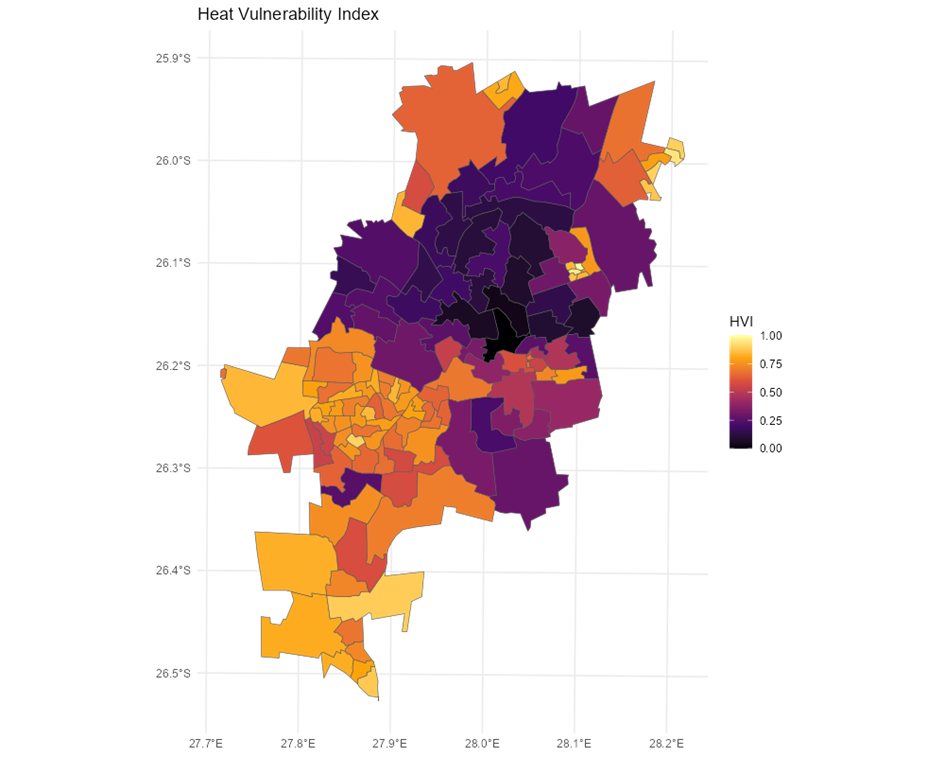
\includegraphics[width=0.8\textwidth]{images/HVI_map_Johannesburg_prelim_analysis.png}
    \caption{Preliminary heat vulnerability index (HVI) map for Johannesburg, integrating socioeconomic, demographic, and environmental factors.}
    \label{fig:hvi}
\end{figure}

\subsection*{A.6 Analytical Framework}
\begin{figure}[H]
    \centering
    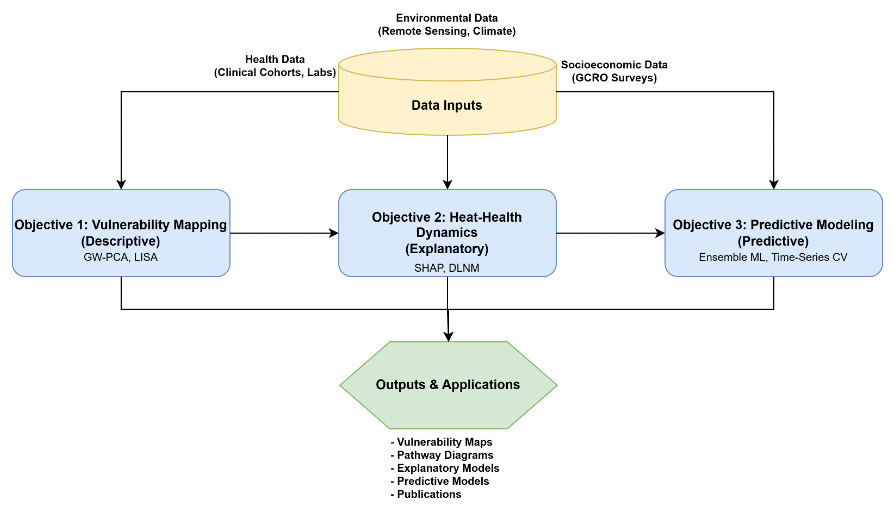
\includegraphics[width=0.7\textwidth]{images/AnalyticalFW.png}
    \caption{Detailed analytical framework showing the integration of vulnerability mapping, heat-health dynamics, and predictive modeling components.}
    \label{fig:analytical}
\end{figure}

\subsection*{F.9 Project Timeline (GANTT Chart)}
\begin{figure}[H]
    \centering
    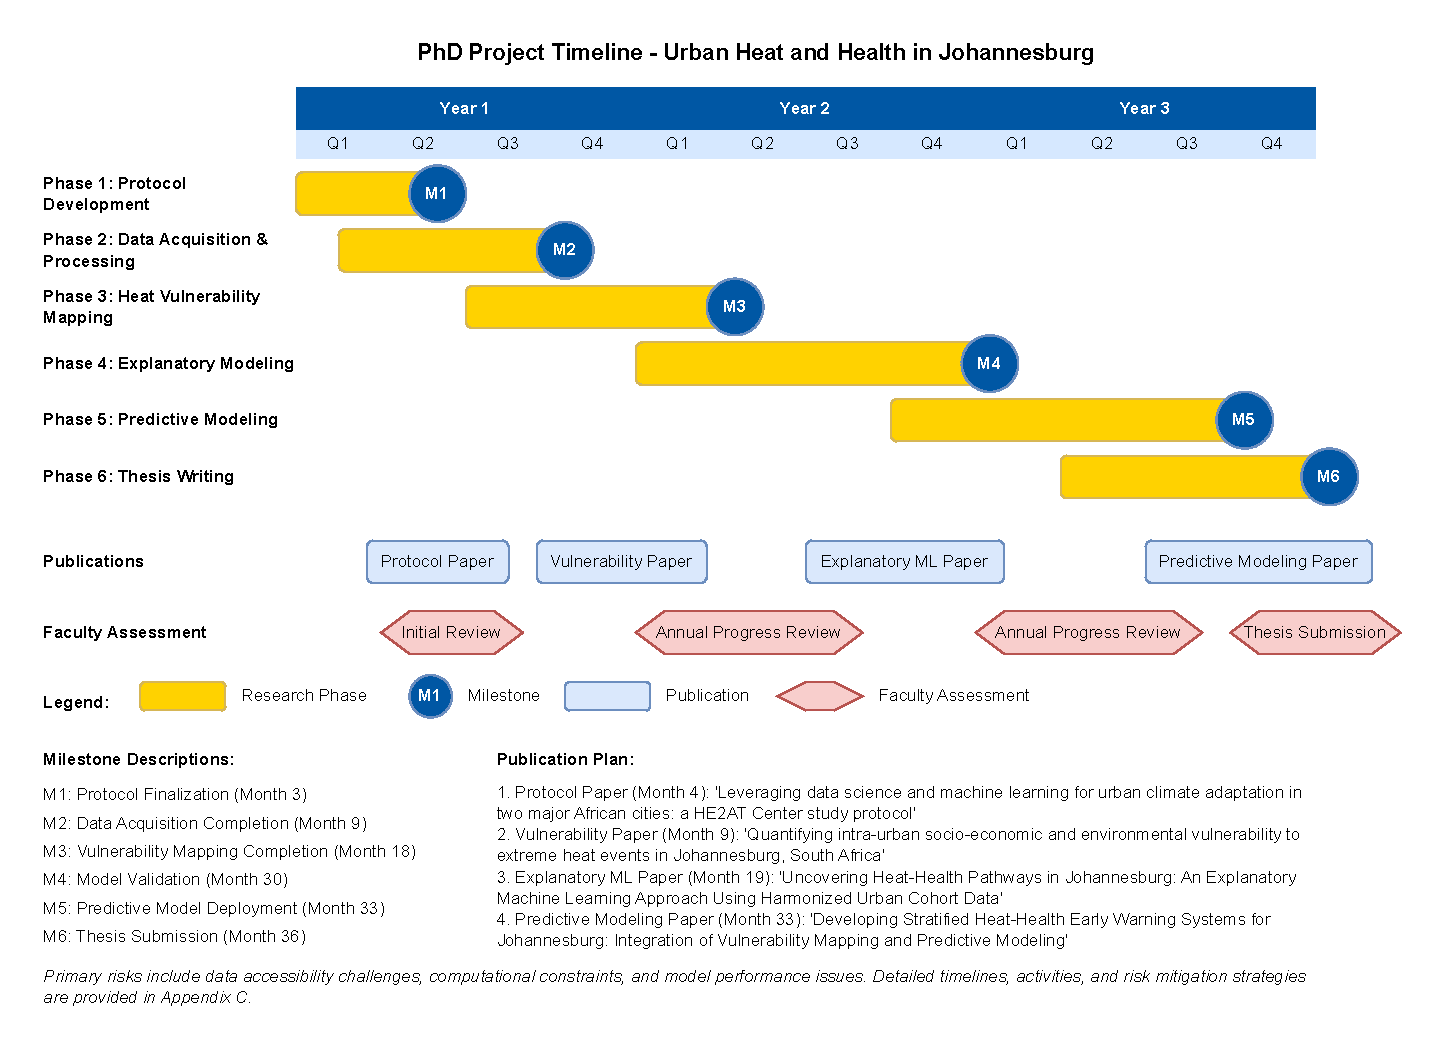
\includegraphics[width=0.9\textwidth]{images/GNT2.drawio.pdf}
    \caption{Detailed project timeline showing research phases, milestones, and deliverables across the PhD duration.}
    \label{fig:gantt}
\end{figure}

\begin{center}
    \Large\textbf{APPENDIX DOCUMENT}\\[0.5em]
    \normalsize\textit{The following tables and appendices are separated from the main document to support word count requirements.}
\end{center}

\section*{Data Management and Methodological Tables for HE\textsuperscript{2}AT Center Research}

\subsection*{Table 1: Key Data Sources for Heat-Health Research}
\begin{longtable}{p{3cm}p{4cm}p{5cm}p{4cm}p{4cm}}
\toprule
\textbf{Data Category} & \textbf{Data Source} & \textbf{Description} & \textbf{Key Variables} & \textbf{Relevance} \\
\midrule
\endhead

\begin{tabular}{c}\textbf{Biomedical}\\\textbf{Data}\end{tabular} 
& Individual Participant Data Platform 
& Collation of prospectively collected high-quality data from pregnant women \& neonates 
& Maternal health indicators, birth outcomes, demographic data 
& Study population with high rates of co-morbidities and adverse health outcomes \\
\midrule

\begin{tabular}{c}\textbf{Climate/Weather}\\\textbf{Data}\end{tabular} 
& ECMWF Forecasts 
& Outputs from numerical weather prediction system 
& Temperature, solar irradiance, wind speed, precipitation, pressure 
& Determination of heat hazard and thermal comfort metrics \\
\cmidrule{2-5}
& ERA5 Reanalysis 
& Global reanalysis dataset combining observed data with meteorological models 
& Temperature, wind speed, precipitation, atmospheric water content 
& Historical climate exposures assessment \\
\cmidrule{2-5}
& ERA5-Land 
& High-resolution land component of the ERA5 climate reanalysis 
& Surface temperature, precipitation, near-surface winds 
& Detailed land surface parameter analysis \\
\midrule

\begin{tabular}{c}\textbf{Remote Sensing}\\\textbf{Data}\end{tabular} 
& SRTM Elevation 
& Global elevation data (30m resolution) 
& Elevation 
& Urban heat island effect assessment \\
\cmidrule{2-5}
& Sentinel-2 Imagery 
& High-resolution multispectral satellite imagery 
& Vegetation coverage, land use classification, NDVI 
& Land cover and urban morphology analysis \\
\cmidrule{2-5}
& MODIS Land Surface Temperature 
& Daily global land surface temperature 
& Day/night land surface temperature 
& Heat exposure assessment \\
\midrule

\begin{tabular}{c}\textbf{Socio-Economic}\\\textbf{Data}\end{tabular} 
& Gauteng City-Region Observatory 
& GIS data for Gauteng City-Region 
& Demographics, economics, environmental factors 
& Socio-economic context for urban areas \\
\cmidrule{2-5}
& South African Census 
& National population and housing census 
& Population density, housing quality, service access 
& Demographic vulnerability factors \\
\cmidrule{2-5}
& GCRO Quality of Life Survey 
& Biennial survey of Gauteng residents 
& Socioeconomic status, health status, service satisfaction 
& Subjective vulnerability factors \\
\bottomrule
\caption{Key Data Sources for Heat-Health Research}
\end{longtable}
\clearpage

\subsection*{Table 2: Data Processing and Integration Workflow}
\begin{longtable}{p{4cm}p{7cm}p{4cm}p{4.5cm}}
\toprule
\textbf{Processing Stage} & \textbf{Key Activities} & \textbf{Responsible Team} & \textbf{Outputs} \\
\midrule
\endhead

\textbf{Pre-processing} 
& Data reformatting, extraction of key variables, alignment with ontologies 
& Core Data Team 
& Standardized data formats ready for harmonization \\
\midrule

\textbf{Variable Mapping} 
& Mapping variables to standardized ontologies, using AI tools for suggestions 
& Harmonization Team 
& Consistent variable naming and definitions across datasets \\
\midrule

\textbf{Mapping Validation} 
& Cross-checking with original data, expert health review 
& Core Data Team, Health Experts 
& Validated variable mappings \\
\midrule

\textbf{Database Population} 
& Application of mappings, transformation of data, de-identification 
& Core Data Team 
& Integrated consortium-shared dataset \\
\midrule

\textbf{Climate Data Integration} 
& Automated retrieval of climate variables, spatial and temporal alignment 
& CSAG/UCT Team 
& Climate-integrated health dataset \\
\midrule

\textbf{De-identification} 
& Safe Harbor method application, expert determination, geographic aggregation 
& Core Data Team 
& RP2 De-identified datasets \\
\midrule

\textbf{Data Analysis} 
& Statistical analysis, machine learning applications 
& HE\textsuperscript{2}AT Consortium 
& Research outputs and inferential data \\
\bottomrule
\caption{Data Processing and Integration Workflow}
\end{longtable}
\clearpage

\subsection*{Table 3: Data Access Levels and Security Measures}
\begin{longtable}{p{3.5cm}p{5cm}p{4.5cm}p{4cm}p{3cm}}
\toprule
\textbf{Data Level} & \textbf{Description} & \textbf{Access Permissions} & \textbf{Security Measures} & \textbf{Retention Period} \\
\midrule
\endhead

\textbf{Original Study Data} 
& Raw, unprocessed health data collected directly from studies 
& Core Data Team only 
& Encryption (AES-256), secure UCT servers, restricted access 
& 5 years after project completion \\
\midrule

\textbf{Consortium Shared Data} 
& Processed, harmonized data with limited indirect identifiers 
& HE\textsuperscript{2}AT Center Consortium partners 
& TLS protocols, access controls, authentication protocols 
& Indefinite (unless specified in DTA) \\
\midrule

\textbf{RP2 De-identified Data} 
& Further de-identified data with aggregated geographic information 
& External Bone Fide Researchers (DAC-approved) 
& Data Transfer Agreements, ethical approval requirements 
& Indefinite (unless specified in DTA) \\
\midrule

\textbf{Inferential Data} 
& Aggregated and anonymized data derived from analyses 
& Open access 
& NA - No identifying information 
& Indefinite \\
\bottomrule
\caption{Data Access Levels and Security Measures}
\end{longtable}
\clearpage

\subsection*{Table 4: Geographic De-identification Techniques}
\begin{longtable}{p{4cm}p{6cm}p{6cm}p{4cm}}
\toprule
\textbf{Technique} & \textbf{Description} & \textbf{Application Scenario} & \textbf{Privacy Protection Level} \\
\midrule
\endhead

\textbf{Geographic Aggregation} 
& Aggregating addresses into larger regions 
& Areas with adequate population density 
& Medium - Depends on aggregation level \\
\midrule

\textbf{Random Direction and Fixed Radius} 
& Points displaced randomly within fixed radius 
& High spatial granularity needs 
& Medium - Predictable displacement bounds \\
\midrule

\textbf{Gaussian Displacement} 
& Random direction with distances following Gaussian distribution 
& Detailed spatial analysis requirements 
& High - Variable displacement with population density \\
\midrule

\textbf{Donut Masking} 
& Setting minimum and maximum displacement levels 
& Preventing both near and far relocations 
& High - Controls minimum displacement \\
\midrule

\textbf{K-anonymity Assessment} 
& Ensuring each location is indistinguishable from k-1 others 
& Validation of masking effectiveness 
& Verification mechanism \\
\bottomrule
\caption{Geographic De-identification Techniques}
\end{longtable}
\clearpage

\subsection*{Table 5: Data Request and Approval Process}
\begin{longtable}{p{3.5cm}p{6cm}p{4.5cm}p{5.5cm}}
\toprule
\textbf{Stage} & \textbf{Description} & \textbf{Responsible Party} & \textbf{Key Considerations} \\
\midrule
\endhead

\textbf{Data Request Submission} 
& Completion of standardized form with research details 
& External Researcher 
& Research purposes, required datasets, ethics approval \\
\midrule

\textbf{Preliminary Screening} 
& Confirmation of form completeness and basic compliance 
& HE\textsuperscript{2}AT Center SteerCo 
& Resource availability, completeness of application \\
\midrule

\textbf{DAC Review} 
& Evaluation based on scientific, ethical, and feasibility criteria 
& Data Access Committee 
& Scientific merit, potential privacy risks, overlap with ongoing research \\
\midrule

\textbf{Decision Communication} 
& Documentation and notification of approval or rejection 
& DAC 
& Transparent reasoning, conditions for approval \\
\midrule

\textbf{Data Transfer} 
& Execution of DTA and data provision 
& Core Data Team 
& Secure transfer protocols, encryption \\
\midrule

\textbf{Ongoing Monitoring} 
& Regular reviews of compliance with agreement terms 
& DAC 
& Audits if necessary \\
\bottomrule
\caption{Data Request and Approval Process}
\end{longtable}

\subsection*{Table 6: Methodological Approaches for Research Objectives}
\begin{table}[H]
\centering
\caption{Methodological Approaches for Research Objectives}
\label{tab:research_objectives}
\begin{tabular}{p{0.3\linewidth}p{0.6\linewidth}}
\toprule
\textbf{Objective} & \textbf{Methodological Approaches} \\
\midrule
\textbf{Vulnerability Mapping} & 
\begin{itemize}[leftmargin=*]
    \item Principal Component Analysis
    \item Geospatial analysis using GIS
    \item Satellite imagery integration
    \item Local Indicators of Spatial Association (LISA)
\end{itemize} \\
\midrule
\textbf{Heat-Health Dynamics} & 
\begin{itemize}[leftmargin=*]
    \item Random Forests for feature importance
    \item XGBoost with SHAP value interpretation
    \item Multi-scale time-series analysis
    \item Physiological pathway investigation
\end{itemize} \\
\midrule
\textbf{Predictive Modeling} & 
\begin{itemize}[leftmargin=*]
    \item Ensemble machine learning approaches
    \item Demographic stratification
    \item Advanced feature selection
    \item Time-series cross-validation
\end{itemize} \\
\bottomrule
\end{tabular}
\end{table}

\subsection*{Table 7: Time-Lag Analysis of Heat-Health Effects}
\begin{table}[H]
\centering
\caption{Time-Lag Analysis of Heat-Health Effects}
\label{tab:time_lag}
\begin{tabular}{p{0.15\linewidth}p{0.35\linewidth}p{0.35\linewidth}}
\toprule
\textbf{Temporal Scale} & \textbf{Health Outcomes} & \textbf{Analytical Approach} \\
\midrule
\textbf{Immediate} \newline(0-24 hours) & 
\begin{itemize}[leftmargin=*]
    \item Cardiovascular responses
    \item Renal function markers
    \item Cognitive performance
\end{itemize} & 
\begin{itemize}[leftmargin=*]
    \item High-resolution temporal analysis
    \item Threshold identification
    \item Diurnal pattern examination
\end{itemize} \\
\midrule
\textbf{Short-term} \newline(1-7 days) & 
\begin{itemize}[leftmargin=*]
    \item Inflammatory markers
    \item Metabolic changes
    \item Sleep quality metrics
\end{itemize} & 
\begin{itemize}[leftmargin=*]
    \item Moving average analysis
    \item Cumulative exposure modeling
    \item Change-point detection
\end{itemize} \\
\midrule
\textbf{Medium-term} \newline(7-30 days) & 
\begin{itemize}[leftmargin=*]
    \item Chronic condition exacerbation
    \item Adaptation responses
    \item Cumulative health impacts
\end{itemize} & 
\begin{itemize}[leftmargin=*]
    \item Distributed lag models
    \item Trend analysis
    \item Physiological pathway assessment
\end{itemize} \\
\bottomrule
\end{tabular}
\end{table}
\clearpage

\section*{Appendix A: Roles and Responsibilities in Data Management}

\begin{longtable}{p{3cm}p{6cm}p{5.5cm}p{5cm}}
\toprule
\textbf{Role} & \textbf{Responsibilities} & \textbf{Current Personnel} & \textbf{Contact} \\
\midrule
\endhead

\textbf{DMAC PIs} 
& Oversight of data management, plan assessment and updates 
& Christopher Jack (UCT), Sibusisiwe Makhanya (IBM) 
& cjack@csag.uct.ac.za, sibusisiwe.makhanya@ibm.com \\
\midrule

\textbf{Health Data Acquisition} 
& Identification of health datasets, DTA development 
& Craig Parker (RP2) 
& Craig.parker@witsphr.org \\
\midrule

\textbf{Core Data Team} 
& Data processing, de-identification, quality control 
& Lisa van Aardenne, Pierre Kloppers, Piotr Wolski, Peter Marsh, Nicholas Brink, Craig Parker 
& Contact DMAC PIs \\
\midrule

\textbf{Data Access Committee} 
& Review of data access requests, oversight of data sharing 
& Caradee Wright (SAMRC), Sibusisiwe Makhanya (IBM), Christopher Jack (UCT) 
& caradee.wright@mrc.ac.za \\
\midrule

\textbf{Information Officer} 
& POPIA compliance, data protection oversight 
& Sibusisiwe Makhanya (IBM) 
& sibusisiwe.makhanya@ibm.com \\
\bottomrule
\caption{Roles and Responsibilities in Data Management}
\end{longtable}
\clearpage

\section*{Appendix B: POPIA Compliance Framework}

\begin{enumerate}[leftmargin=*, itemsep=0.5em]
    \item \textbf{Lawful Processing}: All data processing is conducted exclusively for legitimate research purposes under POPIA Section 27.
    \item \textbf{Purpose Limitation}: Data is collected and processed solely for examining heat-health relationships and vulnerability patterns.
    \item \textbf{Data Minimization}: Only essential data elements required for valid scientific analysis are retained.
    \item \textbf{Information Officer Designation}: A designated Information Officer oversees POPIA compliance with quarterly audits.
    \item \textbf{Security Safeguards}: Technical and organizational measures including encryption, access controls, and secure transfer protocols are implemented.
    \item \textbf{Data Subject Participation}: Where applicable, research participants are informed of data usage through ethics committee-approved processes.
    \item \textbf{Processing Records}: Comprehensive documentation of all data processing activities is maintained.
    \item \textbf{Impact Assessments}: Regular privacy impact assessments are conducted for high-risk processing activities.
\end{enumerate}
\clearpage

\section*{Appendix C: Risk Assessment and Contingency Planning}

\begin{table}[H]
    \centering
    \caption{Risk Assessment and Mitigation Strategies}
    \label{tab:risks}
    \begin{tabular}{p{3cm}p{6cm}p{6cm}}
    \toprule
    \textbf{Risk Category} & \textbf{Potential Issues} & \textbf{Mitigation Strategies} \\
    \midrule
    \textbf{Data Access} & 
    \begin{itemize}[leftmargin=*]
        \item Delays in data acquisition
        \item Restricted access to key datasets
        \item Changes in data provider policies
    \end{itemize} & 
    \begin{itemize}[leftmargin=*]
        \item Early engagement with data providers
        \item Development of alternative data sources
        \item Flexible research design to accommodate data limitations
    \end{itemize} \\
    \midrule
    \textbf{Data Quality} & 
    \begin{itemize}[leftmargin=*]
        \item Missing values in critical variables
        \item Inconsistent data collection methods
        \item Temporal or spatial gaps
    \end{itemize} & 
    \begin{itemize}[leftmargin=*]
        \item Robust imputation methods
        \item Quality assessment protocols
        \item Integration of multiple data sources
    \end{itemize} \\
    \midrule
    \textbf{Computational} & 
    \begin{itemize}[leftmargin=*]
        \item Processing limitations for large datasets
        \item Software compatibility issues
        \item Model convergence failures
    \end{itemize} & 
    \begin{itemize}[leftmargin=*]
        \item Cloud computing resources
        \item Regular code testing and validation
        \item Modular analytical approach
    \end{itemize} \\
    \midrule
    \textbf{Ethical/Legal} & 
    \begin{itemize}[leftmargin=*]
        \item Changes in data protection regulations
        \item Challenges in maintaining anonymization
        \item Stakeholder concerns about findings
    \end{itemize} & 
    \begin{itemize}[leftmargin=*]
        \item Regular compliance reviews
        \item Conservative de-identification approaches
        \item Stakeholder engagement throughout research
    \end{itemize} \\
    \bottomrule
    \end{tabular}
\end{table}

\end{document}
